\documentclass[11pt,a4paper]{article}

\usepackage[margin=2.2cm]{geometry}
\usepackage[T1]{fontenc}
\usepackage{lmodern}
\usepackage{microtype}
\usepackage{amsmath}
\usepackage{amssymb}
\usepackage{graphicx}
\usepackage{booktabs}
\usepackage{caption}
\usepackage{subcaption}
\usepackage{float}
\usepackage{enumitem}
\usepackage{xcolor}
\usepackage[hidelinks]{hyperref}

% Figures: reports/figures in the repository, figures/ on Overleaf.
\graphicspath{{figures/}{../reports/figures/}}
\setlist{nosep, leftmargin=*}
\captionsetup{font=small, labelfont=bf}
\setlength{\parskip}{0.35em}
\setlength{\parindent}{0pt}

\newcommand{\eur}[1]{EUR~#1}
% Decision / Why / Risk box closing each section.
\newcommand{\dwr}[3]{\par\smallskip\noindent\colorbox{gray!10}{\parbox{\dimexpr\linewidth-2\fboxsep}{\small
\textbf{Decision.} #1\\ \textbf{Why.} #2\\ \textbf{Risk.} #3}}\par\smallskip}

\title{\textbf{Who should the bank call?}\\[0.3em]
\large Dataset: \textbf{Bank Marketing} (UCI, OpenML id 1461)}
\author{Khaled Elnagar \quad Alzira Ferreira\\[0.3em]
\small MSc, \emph{Supervised Learning \& Model Engineering}, Albert School, October 2026\\
\small Code: \url{https://github.com/khaledngr/bank-marketing-project}}
\date{}

\begin{document}
\maketitle
\vspace{-2.2em}

\begin{abstract}
\noindent A bank phones clients to sell a term deposit; 11.7\% of 45,211 clients subscribe. A call
costs \eur{5}, a subscription earns \eur{50}. We built a leakage-free pipeline from raw data to a
served prediction endpoint. A tuned LightGBM reaches an average precision (AP) of 0.476 on an
untouched test set (random: 0.117). Calling the 24\% of clients above a profit-optimal threshold
reaches 67\% of subscribers and earns \eur{2,711} per 1,000 clients, 3.2$\times$ more than calling
everyone. Probabilities are well calibrated (ECE 0.010), but a time-ordered check shows they go
stale when the base rate shifts. Age-group thresholds close an equal-opportunity gap from 35 to 5
points at a cost of 6\% of profit.
\end{abstract}

%=====================================================================
\section{Problem framing and data}

\begin{itemize}
  \item \textbf{Task:} before calling, predict $p = P(\text{subscribe})$ from what the bank already
  knows (profile, balance, loans, contact history).
  \item \textbf{Decision rule:} call if $p \times 50 > 5$, i.e.\ $p > 0.10$. Costs are our assumptions
  (\texttt{config.yaml}).
  \item \textbf{Data:} 45,211 clients, 16 features; target \texttt{Class}$=2$ mapped to $y=1$
  (checked against the documented 11.7\%). No missing cells, no duplicates; missing information hides
  in \texttt{unknown} (\texttt{contact}: 29\%) and \texttt{pdays}$=-1$ (``never contacted'', 82\%).
  \item \textbf{Split:} stratified 80/20 with a fixed seed. Test set (9,043) scored once at the end;
  validation = stratified 5-fold CV on the 80\%, same folds for every model. EDA on training data only.
\end{itemize}

\begin{figure}[H]
\centering
\begin{subfigure}{0.62\textwidth}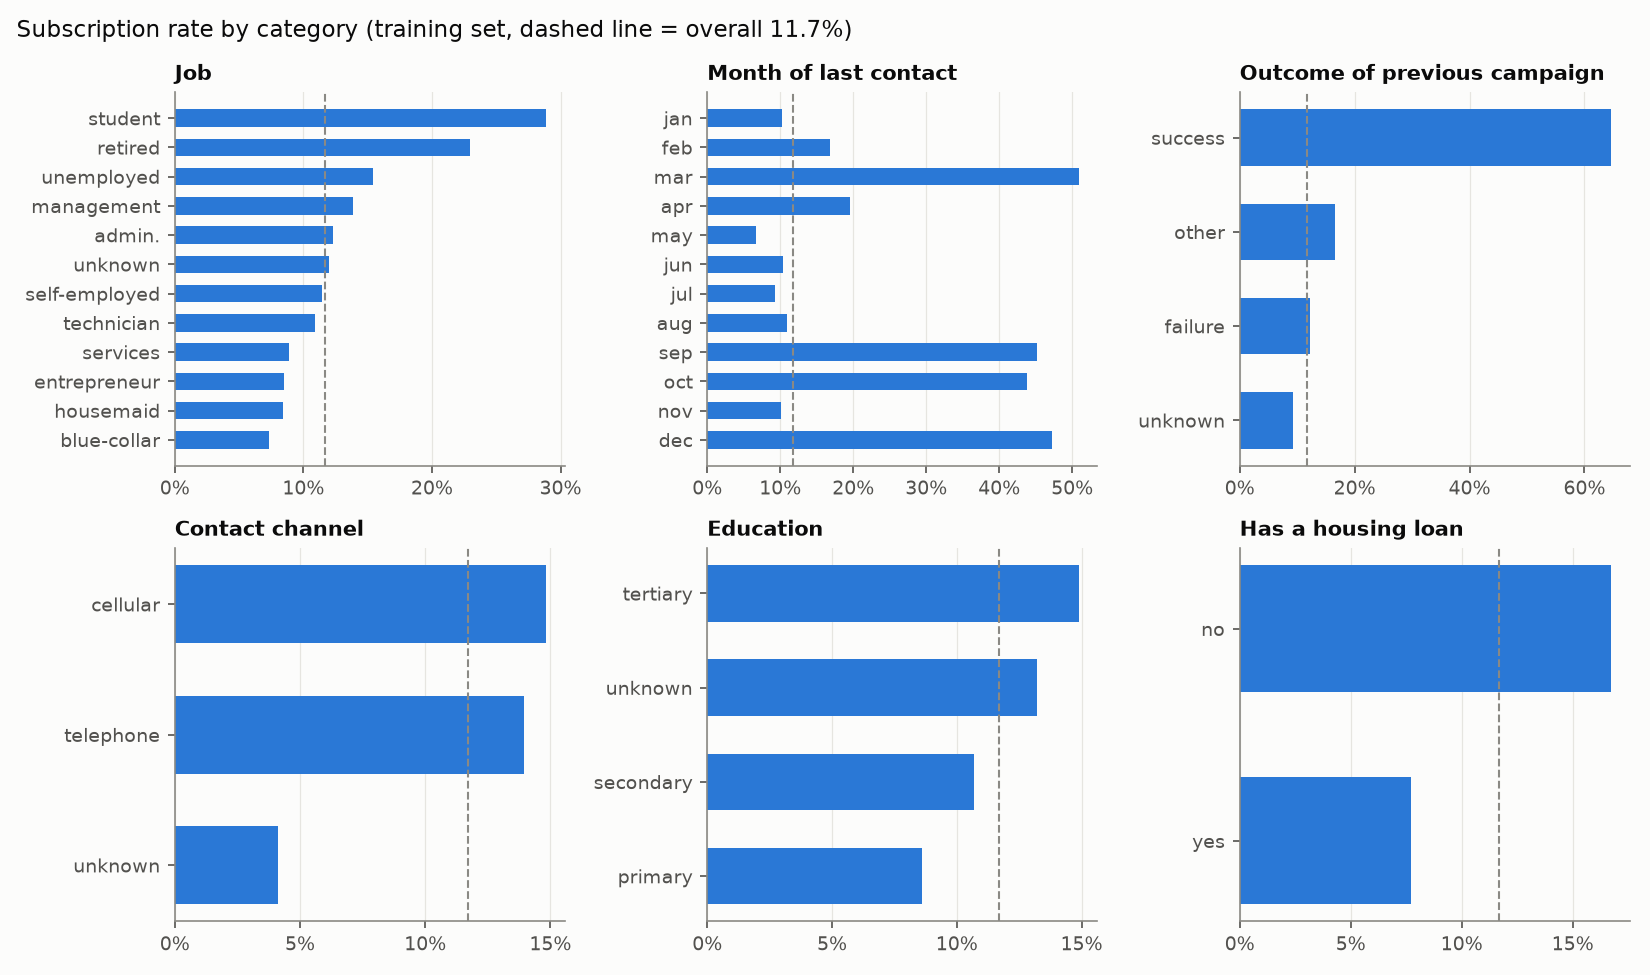
\includegraphics[width=\linewidth]{eda_categorical_rates}\end{subfigure}
\begin{subfigure}{0.36\textwidth}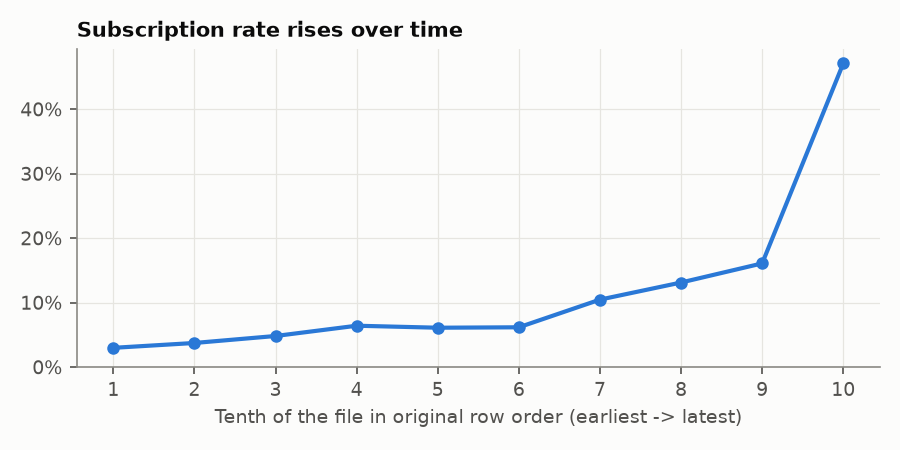
\includegraphics[width=\linewidth]{eda_drift_by_row_order}\end{subfigure}
\caption{Left: subscription rate by category (dashed = 11.7\%). Right: rate along the file, which UCI
documents as ordered by date (May 2008 -- Nov 2010).}
\label{fig:eda}
\end{figure}

\dwr{Drop \texttt{duration} (call length) before any split.}
{It is only known after the call (calls $<$ 90 s convert at 0.7\%, $>$ 6 min at 33\%): pure leakage.}
{Time drift: the rate rises from 3\% to 47\% along the file and the split is random, so the test
score describes clients from the same period, not a future campaign (quantified by a time-ordered
check, Section~\ref{sec:final}). No client ID: repeated clients across the split cannot be ruled out.}

%=====================================================================
\section{Feature engineering}

Inside the Pipeline, refitted in every fold: median imputation + scaling for numbers, one-hot encoding
for categories (\texttt{unknown} kept as a category: \texttt{contact}=unknown converts at 4\% vs.\ 15\%
for cellular). Three rule-based features (no fitted statistics, so no leakage):
\begin{itemize}
  \item \texttt{contacted\_before}: flags \texttt{pdays}$=-1$, which is then imputed instead of read
  as ``1 day ago''.
  \item Logarithms of \texttt{balance} (signed), \texttt{campaign}, \texttt{previous}: long tails
  (balance up to \eur{102,127}).
  \item \texttt{life\_stage} ($<25$ / 25--59 / $\geq 60$): subscription is U-shaped in age (26\%, 10\%, 34\%).
\end{itemize}

\begin{table}[H]
\centering\small
\begin{tabular}{lcc}
\toprule
Features (cumulative) & Logistic regression AP & LightGBM AP \\
\midrule
Raw columns & 0.402 & 0.445 \\
+ \texttt{contacted\_before} & 0.402 & 0.449 \\
+ logarithms & 0.406 & 0.447 \\
+ \texttt{life\_stage} & 0.408 & 0.449 \\
\bottomrule
\end{tabular}
\caption{Feature ablation, mean AP over 5 CV folds (fold std $\approx$ 0.01).}
\label{tab:ablation}
\end{table}

\dwr{Keep the three features: cheap, interpretable, and they never lower AP.}
{Linear model gains +0.006 AP (it cannot bend on its own); trees gain nothing measurable (they find
thresholds and U-shapes themselves).}
{Gains are within fold noise. \texttt{life\_stage} derives from age, the sensitive attribute (Section~\ref{sec:fairness}).}

%=====================================================================
\section{Class imbalance}\label{sec:imbalance}

Accuracy is uninformative (``never call'' is 88\% accurate). Metrics: \textbf{AP} (ranking of the rare
class; random = 0.117), \textbf{precision} (calls that convert), \textbf{recall} (subscribers reached)
and \textbf{profit}. Remedies compared on LightGBM inside the folds; class weights computed per training
fold, SMOTE inside an \texttt{imblearn} Pipeline. Thresholds chosen on out-of-fold scores.

\begin{table}[H]
\centering\small
\begin{tabular}{llccccc}
\toprule
Remedy & Threshold & AP & Precision & Recall & Called & Profit / 1,000 \\
\midrule
None & 0.50 (default) & 0.449 & 0.62 & 0.25 & 5\% & \eur{1,213} \\
\textbf{None} & \textbf{0.11 (profit)} & \textbf{0.449} & 0.32 & 0.65 & 24\% & \textbf{\eur{2,638}} \\
Class weights & 0.44 (profit) & 0.446 & 0.29 & 0.67 & 27\% & \eur{2,606} \\
SMOTE & 0.16 (profit) & 0.432 & 0.29 & 0.66 & 27\% & \eur{2,512} \\
\midrule
Call everyone & -- & 0.117 & 0.12 & 1.00 & 100\% & \eur{849} \\
\bottomrule
\end{tabular}
\caption{Imbalance remedies (default LightGBM, 5-fold CV).}
\label{tab:imbalance}
\end{table}

\begin{figure}[H]
\centering
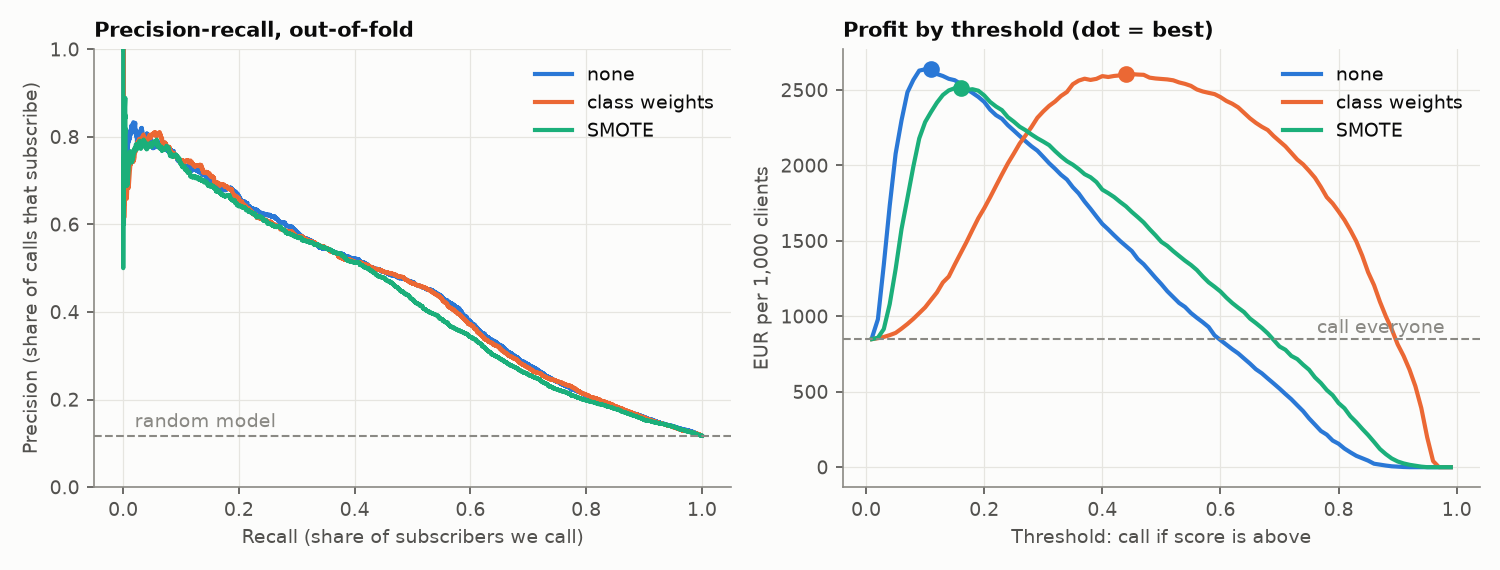
\includegraphics[width=0.9\textwidth]{imbalance_pr_and_profit}
\caption{Left: precision--recall curves. Right: profit per 1,000 clients by threshold (dot = best;
dashed = call everyone).}
\label{fig:imbalance}
\end{figure}

\dwr{Cost-based threshold (0.11); no class weights, no SMOTE.}
{Weights and SMOTE do not improve AP and both distort probabilities: mean prediction 36\% with
weights (ECE 0.24) and 16\% with SMOTE (ECE 0.04), vs.\ 11.6\% (ECE 0.006) plain, for 11.7\% observed.
SMOTE also interpolates one-hot columns (SMOTENC would not, but SMOTE already loses). The threshold
doubles profit vs.\ 0.5 and lands next to the break-even 0.10.}
{Threshold chosen on the same out-of-fold scores we report (checked on test). Profit depends on the
assumed costs; the profit curve is flat between 0.09 and 0.15 (Figure~\ref{fig:imbalance}).}

%=====================================================================
\section{Models, Pipeline and tuning}\label{sec:models}

One scikit-learn Pipeline, used for CV, tuning, explanation and serving:
\emph{features} $\rightarrow$ \emph{ColumnTransformer} $\rightarrow$ \emph{model}. Refitting the
whole object per fold means no statistic is learned from validation clients. Tuning: Optuna (TPE,
seed 42), 30 trials per model, each scored by mean AP on the same 5 folds; search spaces in
Appendix~\ref{app:params}. All runs are tracked in MLflow (Section~\ref{sec:tracking}).

\begin{table}[H]
\centering\small
\begin{tabular}{lccccccc}
\toprule
& \multicolumn{2}{c}{AP} & \multicolumn{2}{c}{Profit / 1,000} & \multicolumn{3}{c}{Tuned, at profit threshold} \\
\cmidrule(lr){2-3}\cmidrule(lr){4-5}\cmidrule(lr){6-8}
Model & default & tuned & default & tuned & Thr. & Prec. & Recall \\
\midrule
Call everyone & 0.117 & -- & \eur{849} & -- & -- & 0.12 & 1.00 \\
Logistic regression (baseline) & 0.408 & 0.409 & \eur{2,347} & \eur{2,366} & 0.13 & 0.30 & 0.61 \\
Random forest & 0.412 & 0.448 & \eur{2,525} & \eur{2,613} & 0.12 & 0.32 & 0.65 \\
\textbf{LightGBM} & \textbf{0.449} & \textbf{0.459} & \eur{2,638} & \textbf{\eur{2,676}} & 0.11 & 0.32 & 0.66 \\
\bottomrule
\end{tabular}
\caption{Three models, same folds, same metrics (5-fold CV; AP fold std 0.010--0.017).}
\label{tab:models}
\end{table}

\begin{figure}[H]
\centering
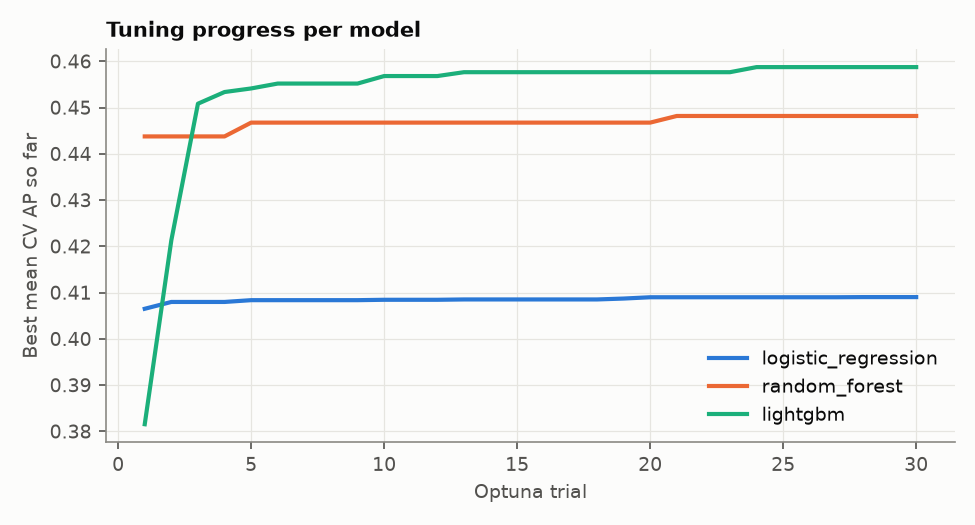
\includegraphics[width=0.55\textwidth]{tuning_history}
\caption{Optuna: best mean CV AP so far per trial; most of the gain comes in the first 10--20 trials.}
\label{fig:tuning}
\end{figure}

\textbf{What each step bought.}
\begin{itemize}
  \item No model $\rightarrow$ logistic regression: AP 0.117 $\rightarrow$ 0.408, profit $\times$2.8.
  \item $\rightarrow$ random forest: finds interactions; gains most from tuning (+0.036 AP: min leaf 4,
  20\% of features per split, i.e.\ less overfit, more diverse trees).
  \item $\rightarrow$ LightGBM: best AP and profit; tuned to learning rate 0.013 with 560 trees.
  \item Logistic regression barely tunes (+0.001): limited by its linear form; Optuna leaned to Lasso
  (\texttt{l1\_ratio} 0.85).
\end{itemize}

\dwr{Tuned LightGBM as final model.}
{Best AP, ROC-AUC and profit; the course's working model.}
{Its lead over a tuned random forest ($\approx$ 0.011 AP) is about one fold std. The same folds select
and score, so we checked with nested CV (\texttt{src/nested\_cv.py}: 5 outer folds, 15 Optuna trials
and the threshold chosen inside each): AP 0.458 $\pm$ 0.012 and \eur{2,667} vs.\ 0.459 and \eur{2,676},
threshold 0.10--0.11 in every fold, so the selection bias is negligible. Tree count was tuned instead
of early stopping, which would need an extra split inside each fold.}

%=====================================================================
\section{Experiment tracking}\label{sec:tracking}

MLflow (local SQLite store). One parent run per experiment with its tables and figures as artifacts;
one child run per candidate with all parameters, metrics, per-fold AP and the git commit. Covered:
feature ablation, imbalance remedies, model comparison, 90 Optuna trials (plus each study's trial
table), explainability, calibration, fairness, the final model (logged as an MLflow model) and the
two supplementary checks. Fixed seeds: re-running the scripts rebuilds identical runs. The store itself
(\texttt{mlflow.db}) is not committed, so a reader rebuilds it by running the scripts ($\approx$ 20 min);
Optuna trials carry parameters and metrics, artifacts are kept per study.

\begin{figure}[H]
\centering
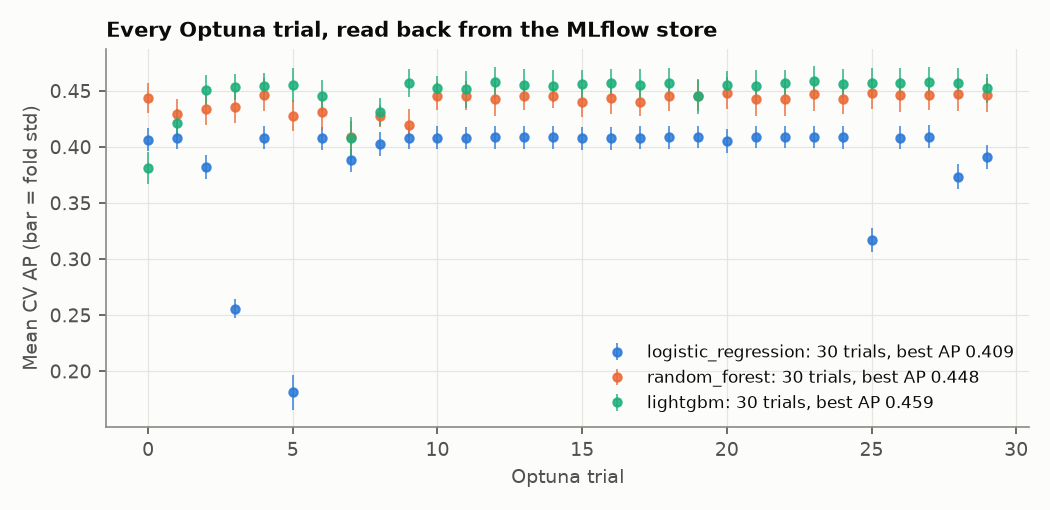
\includegraphics[width=0.75\textwidth]{mlflow_trials}
\caption{All 90 Optuna trials, read back from the MLflow store (\texttt{python -m src.tracking}):
mean CV AP per trial, bar = fold standard deviation.}
\label{fig:mlflow}
\end{figure}

%=====================================================================
\section{Explainability}

Tuned LightGBM fitted on 4 folds, explained on the 5th (7,234 unseen clients): same settings as the
deployed model but not the deployed fit, so the test set stays untouched. Three global views:
\textbf{gain} (training improvement), \textbf{permutation} (validation AP lost when shuffled; 10 repeats;
\texttt{pdays}/\texttt{previous}/\texttt{poutcome} shuffled together) and \textbf{mean $|$SHAP$|$}
(log-odds contribution).

\begin{figure}[H]
\centering
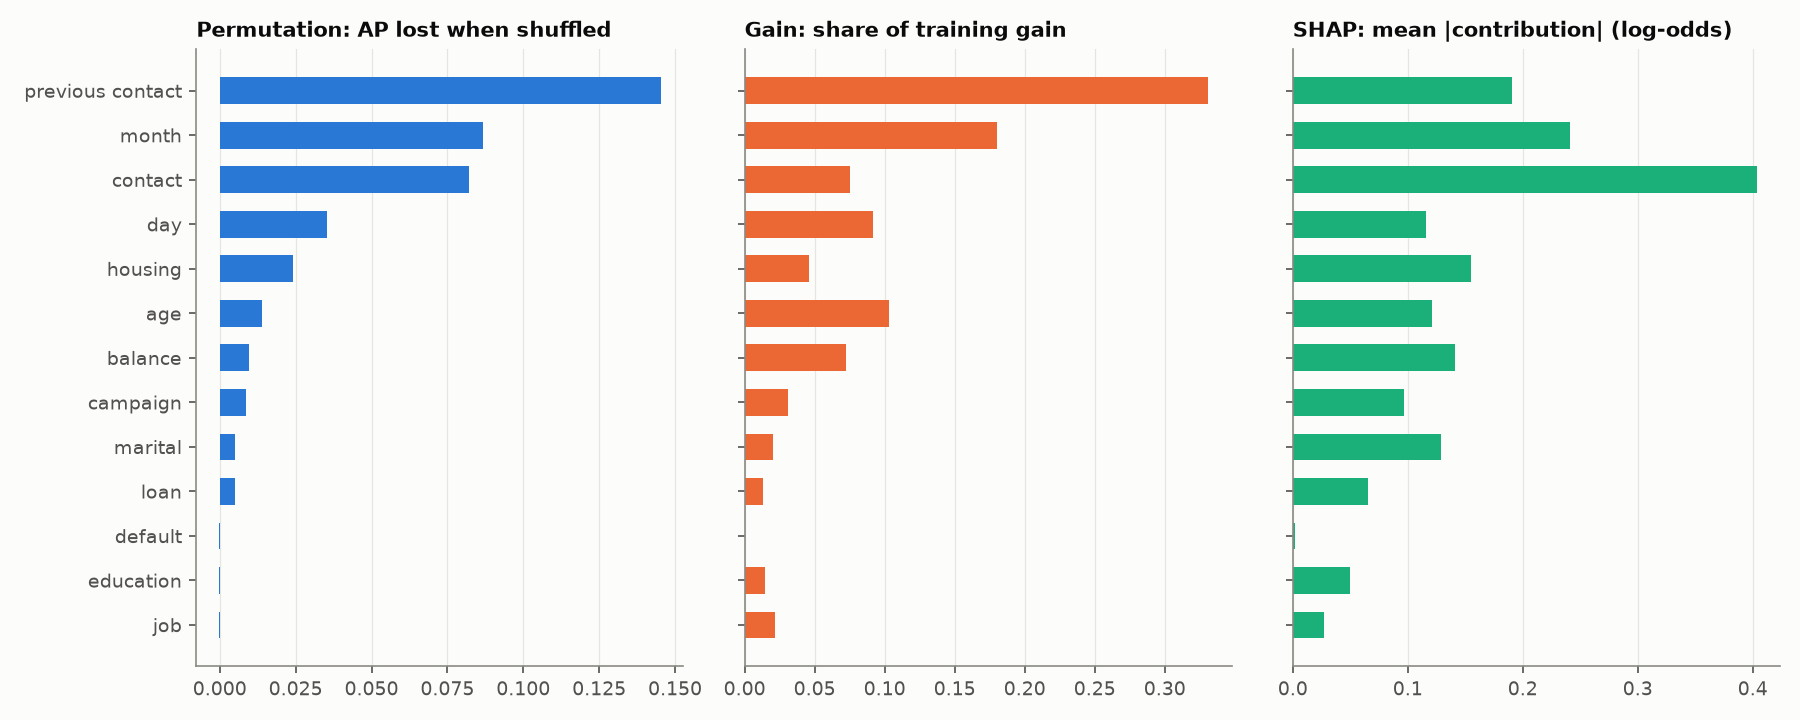
\includegraphics[width=0.95\textwidth]{importance_three_views}
\caption{Global importance, aggregated to client variables.}
\label{fig:importance}
\end{figure}

\begin{figure}[H]
\centering
\begin{subfigure}{0.49\textwidth}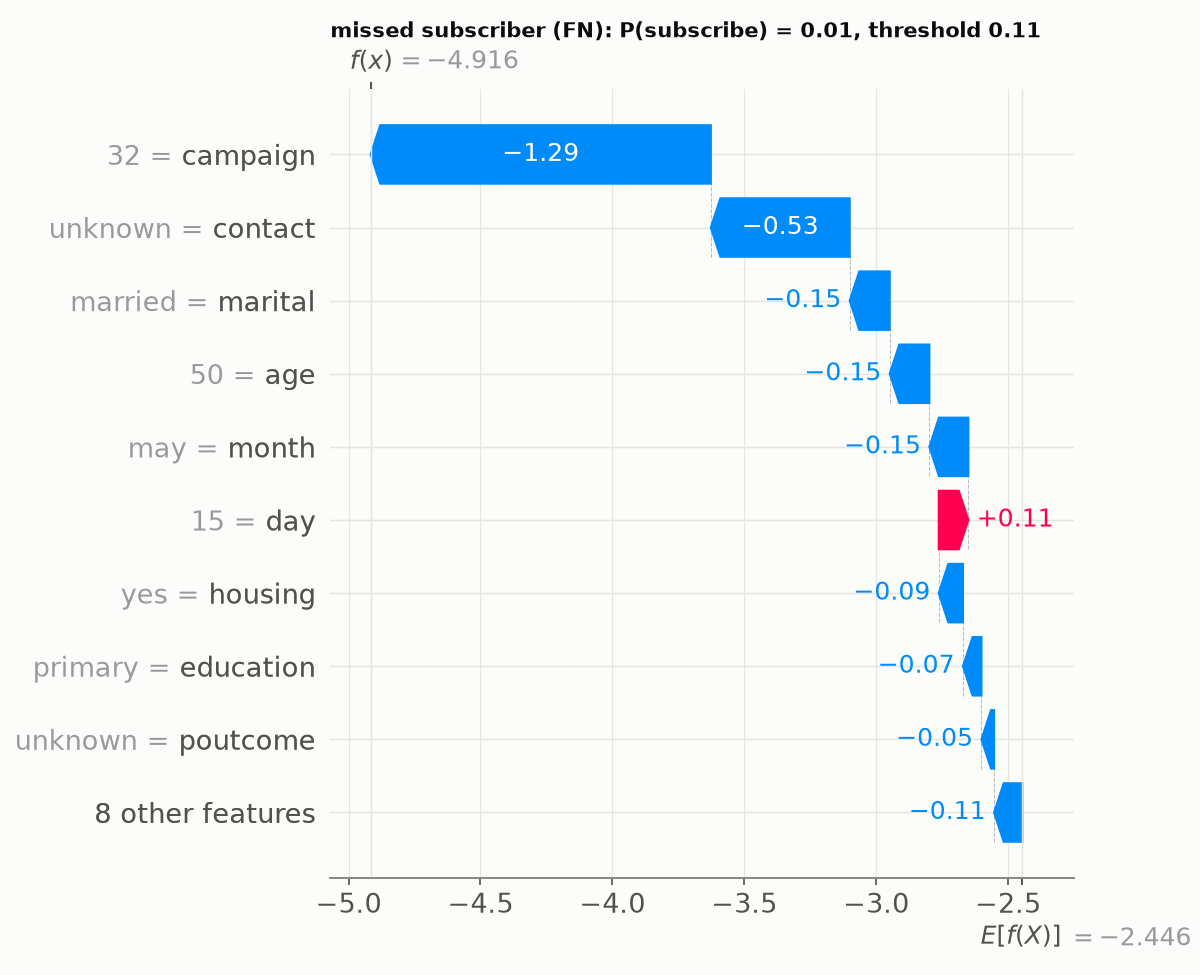
\includegraphics[width=\linewidth]{shap_local_FN}\end{subfigure}
\begin{subfigure}{0.49\textwidth}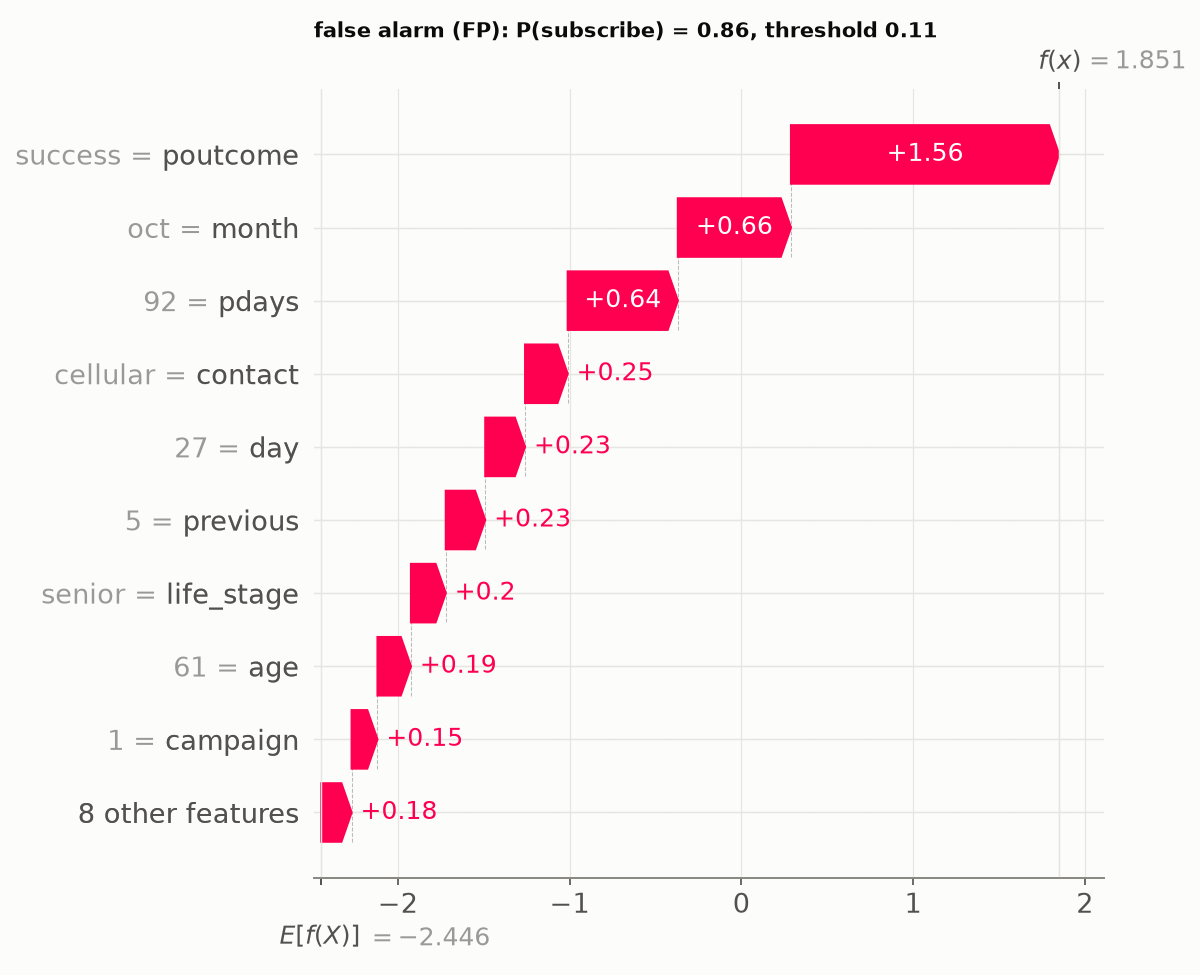
\includegraphics[width=\linewidth]{shap_local_FP}\end{subfigure}
\caption{Local SHAP (log-odds). Left: missed subscriber, $p$ = 0.007, already called 32 times.
Right: false alarm, $p$ = 0.86, retiree with a previous success.}
\label{fig:local}
\end{figure}

\textbf{Business sense.}
\begin{itemize}
  \item Previous campaign outcome dominates (AP $-0.145$ when shuffled): past buyers buy again. \checkmark
  \item Housing loan $\downarrow$, higher balance $\uparrow$, many calls this campaign $\downarrow$, age U-shape. \checkmark
  \item Job, education, default $\approx 0$: their information is already carried by the rest.
  \item \texttt{month}, \texttt{contact} and \texttt{day} partly encode \emph{when} the call happened
  (drift): \texttt{contact}=unknown fills the first 28\% of the file (2008) and almost nothing after,
  and \texttt{day} (day of month) has no client meaning. Treat these as timing, not behaviour.
  \item Views disagree as expected: \texttt{contact} is \#1 by SHAP but \#3 by permutation
  (\texttt{month} substitutes when it is shuffled); age is high by gain (training-based, favours
  continuous features) but low by permutation.
\end{itemize}

\dwr{Report all three views and four local cases (two more in Appendix~\ref{app:figures}).}
{Each view answers a different question; local cases show the model's logic, e.g.\ ``stop after 32 calls'' is rational at \eur{5} per call.}
{SHAP explains the model, not causes. Correlated features share or swap importance.}

%=====================================================================
\section{Calibration}\label{sec:calibration}

The call rule needs honest probabilities. Compared on out-of-fold scores: uncalibrated, Platt
(sigmoid) and isotonic, the latter two via \texttt{CalibratedClassifierCV} on inner folds (no
calibrator sees its own training labels).

\begin{table}[H]
\centering\small
\begin{tabular}{lccccc}
\toprule
Candidate & AP & Brier & ECE (10 bins) & Mean predicted & Profit / 1,000 \\
\midrule
\textbf{Uncalibrated} (CV) & 0.459 & 0.0811 & 0.006 & 11.6\% & \eur{2,676} \\
Platt (CV) & 0.458 & 0.0811 & 0.006 & 11.7\% & \eur{2,667} \\
Isotonic (CV) & 0.458 & 0.0810 & 0.003 & 11.7\% & \eur{2,651} \\
\textbf{Uncalibrated (test)} & 0.476 & 0.0798 & 0.010 & -- & \eur{2,711} \\
\bottomrule
\end{tabular}
\caption{Probability quality (observed rate 11.7\%).}
\label{tab:calibration}
\end{table}

\begin{figure}[H]
\centering
\begin{subfigure}{0.42\textwidth}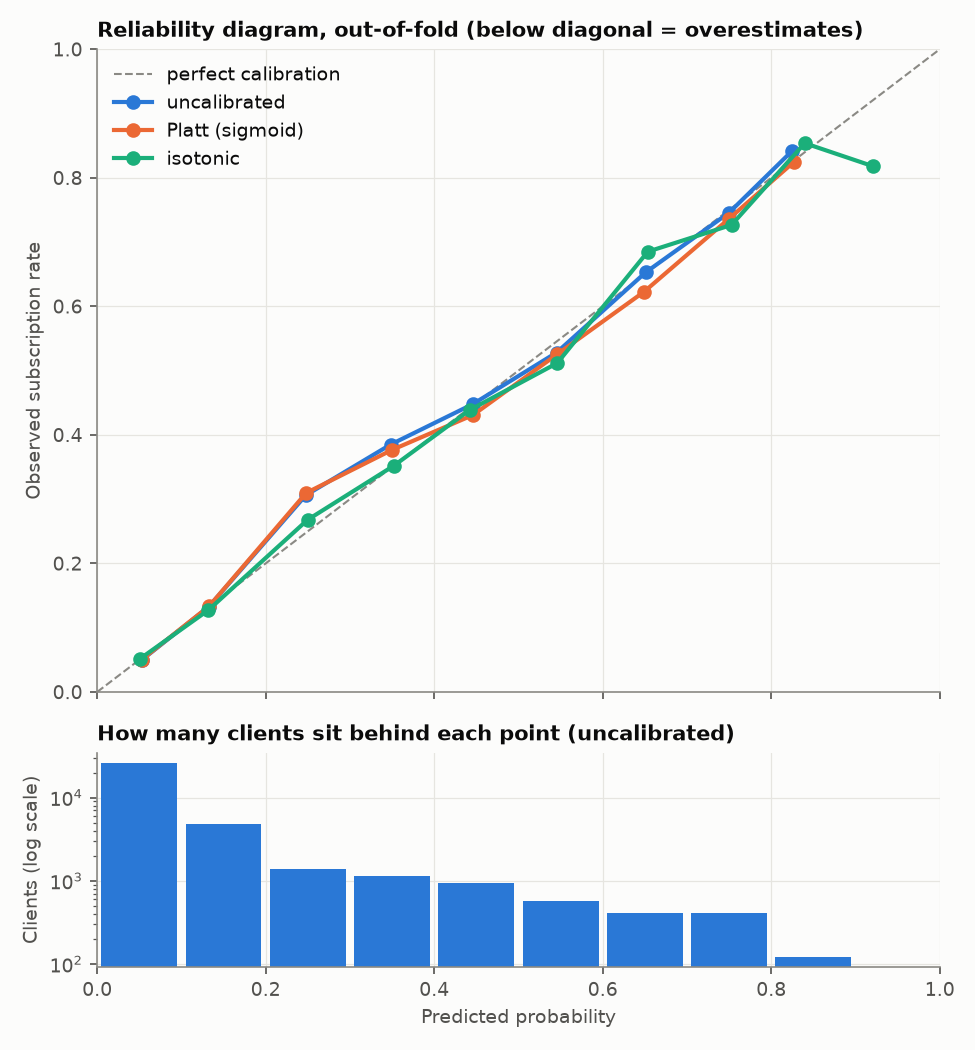
\includegraphics[width=\linewidth]{calibration_reliability}\end{subfigure}
\begin{subfigure}{0.42\textwidth}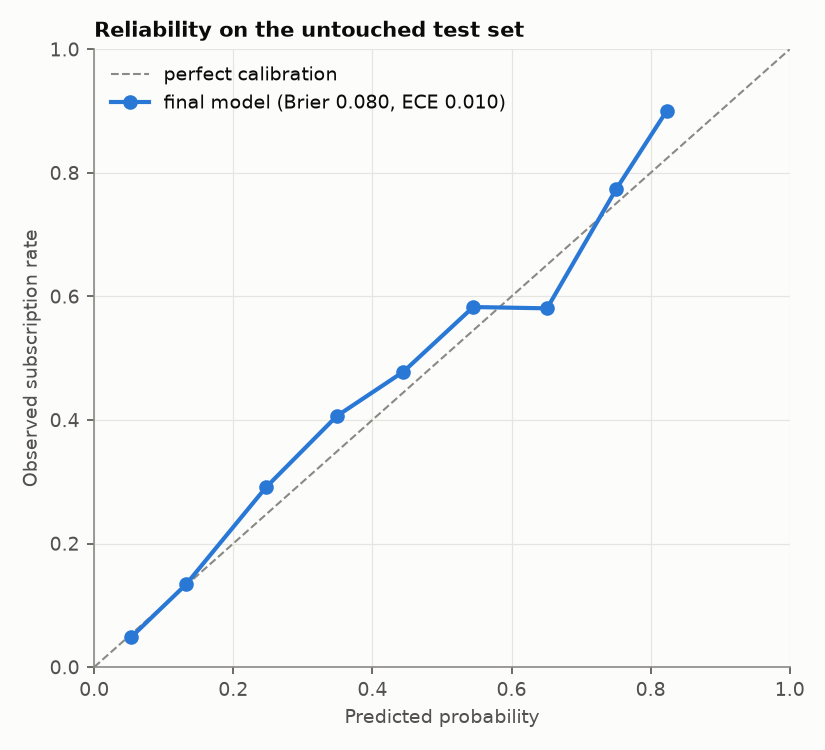
\includegraphics[width=\linewidth]{final_test_reliability}\end{subfigure}
\caption{Reliability diagrams. Left: CV with clients per bin. Right: test set.}
\label{fig:calibration}
\end{figure}

\dwr{Keep the model uncalibrated; trust its probabilities for the call rule.}
{Already calibrated: in the 10--20\% bin, where decisions are made, predicted = observed = 13.2\%.
Brier 0.081 vs.\ 0.103 for always predicting 11.7\% (skill score 0.22).
Slightly under-confident at 20--40\% (predicts 25\%, observes 31\%). Isotonic halves ECE but not Brier
and lowers profit: simpler wins. Log-loss training and no reweighting (Section~\ref{sec:imbalance}) keep it honest.}
{Calibration goes stale under drift; group-level calibration differs (ECE 0.010--0.049 per age group on test).}

%=====================================================================
\section{Fairness audit on age}\label{sec:fairness}

\begin{itemize}
  \item \textbf{Groups:} young ($<25$), working (25--59), senior ($\geq 60$): the U-shape of the data,
  same cut-offs as \texttt{life\_stage}.
  \item \textbf{Definition: equal opportunity} (equal recall). Harm = an interested client never
  offered the product. Demographic parity does not fit: interest differs by age (26\% / 10\% / 34\%),
  and with different base rates the definitions cannot all hold.
  \item \textbf{Audit (CV):} recall 0.90 / 0.61 / 0.97, 95\% Wilson intervals do not overlap. Removing
  age barely helps (gap 36 $\rightarrow$ 29 points; \texttt{job} = retired/student are proxies) and
  worsens senior calibration (ECE 0.027 $\rightarrow$ 0.056).
  \item \textbf{Mitigation (post-processing):} per-group thresholds set on out-of-fold scores to reach
  the overall recall (0.66): 0.34 / 0.09 / 0.33. Model unchanged. Frozen, then applied to the test set:
\end{itemize}

\begin{table}[H]
\centering\small
\begin{tabular}{llccccc}
\toprule
Test set & Group & Subscribers & Called & Recall [95\% CI] & Unwanted calls & Precision \\
\midrule
One threshold & young & 39 & 68\% & 0.95 [0.83, 0.99] & 58\% & 0.36 \\
(0.11) & working & 907 & 21\% & 0.62 [0.59, 0.65] & 16\% & 0.31 \\
 & senior & 112 & 82\% & 0.97 [0.92, 0.99] & 75\% & 0.39 \\
\midrule
Age-group & young & 39 & 30\% & 0.64 [0.48, 0.77] & 19\% & 0.54 \\
thresholds & working & 907 & 29\% & 0.69 [0.66, 0.72] & 24\% & 0.25 \\
 & senior & 112 & 42\% & 0.69 [0.60, 0.77] & 29\% & 0.54 \\
\bottomrule
\end{tabular}
\caption{Fairness on the test set. Recall gap 35 $\rightarrow$ 5 points; profit \eur{2,711}
$\rightarrow$ \eur{2,551} per 1,000 clients ($-6\%$).}
\label{tab:fairness}
\end{table}

\begin{figure}[H]
\centering
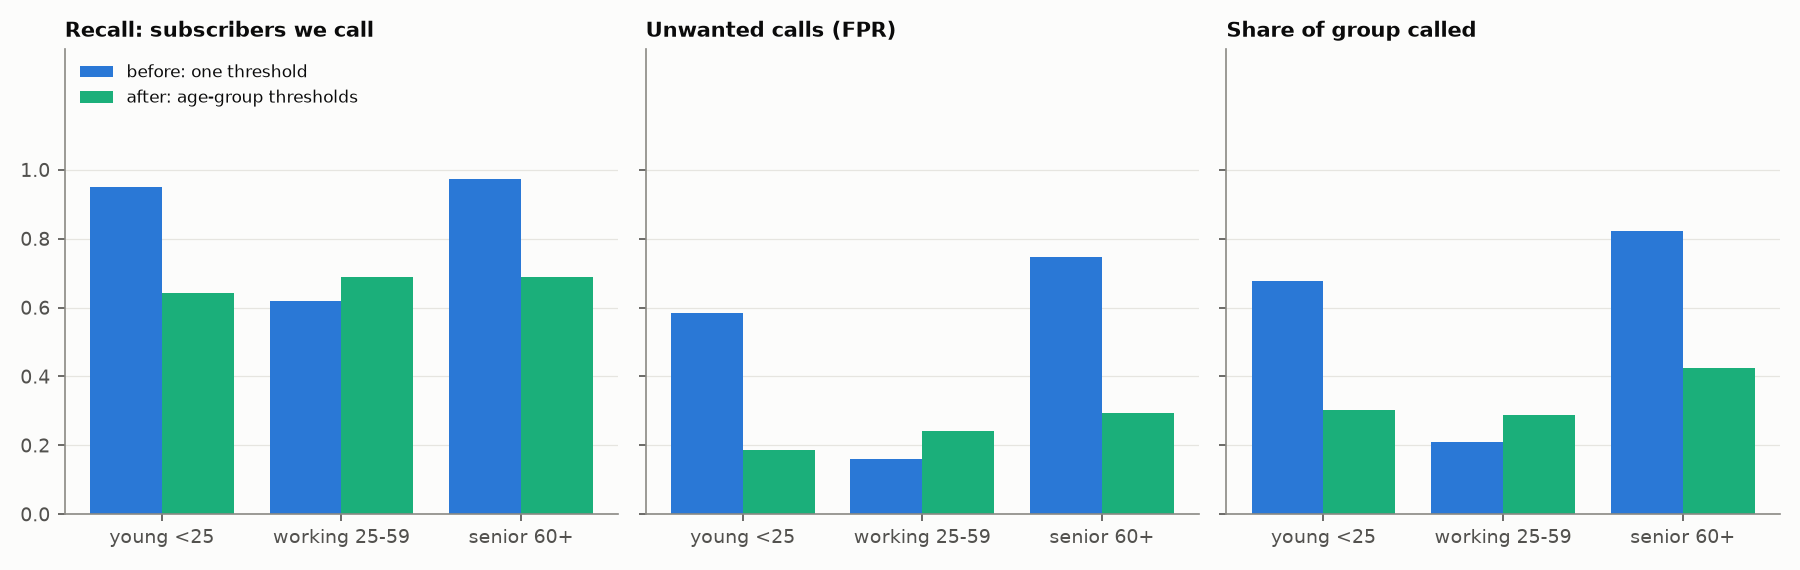
\includegraphics[width=0.9\textwidth]{final_test_fairness}
\caption{Test set, per age group: recall, unwanted calls and share called, before and after mitigation.}
\label{fig:fairness}
\end{figure}

\dwr{Report both policies; the API returns both decisions.}
{Mitigation closes the equal-opportunity gap (intervals overlap). Fewer unwanted calls to seniors
(75\% $\rightarrow$ 29\%) is a side effect, not the criterion.}
{$-6\%$ profit; levelling down: the gap closes mostly by calling fewer young and senior clients, which
skips calls worth $+$\eur{11.5} at $p = 0.33$; precision gap grows (0.25 vs.\ 0.54), i.e.\ predictive
parity breaks; only 39 young subscribers in test (recall CI 0.48--0.77), so the small gap is not
statistically established; using age explicitly is disparate treatment, a legal choice for the bank
(EU).}

%=====================================================================
\section{Final evaluation and deployment}\label{sec:final}

All choices frozen on CV; Pipeline refitted on the 36,168 training clients; test set scored once.

\begin{table}[H]
\centering\small
\begin{tabular}{lccc}
\toprule
& CV & \textbf{Test} & Test: call everyone \\
\midrule
AP / ROC-AUC & 0.459 / 0.802 & \textbf{0.476 / 0.809} & 0.117 / 0.500 \\
Precision / recall at 0.11 & 0.32 / 0.66 & 0.33 / 0.67 & 0.12 / 1.00 \\
Clients called & 24\% & 24\% & 100\% \\
Profit per 1,000 clients & \eur{2,676} & \textbf{\eur{2,711}} & \eur{850} \\
Brier / ECE & 0.081 / 0.006 & 0.080 / 0.010 & -- \\
\bottomrule
\end{tabular}
\caption{Final model on the untouched test set (9,043 clients).}
\label{tab:final}
\end{table}

\textbf{Served endpoint.} FastAPI app loading the saved Pipeline and thresholds. \texttt{POST /predict}
takes one client's raw fields (validated categories, age 18--100, no \texttt{duration}) and returns
$p$, the expected value $50p - 5$, and the business and age-fair decisions. Raw inputs go through the
same fitted preprocessing as in training.

\dwr{Ship the tuned LightGBM with threshold 0.11 behind the API.}
{Test matches CV (AP 0.476 vs.\ 0.459, within fold noise); 3.2$\times$ the profit of calling everyone;
one call in three converts vs.\ one in eight at random.}
{Same-period test set; proof of concept without authentication, batch scoring or monitoring of
drift and calibration.}

\textbf{Supplementary time-ordered check} (\texttt{src/temporal.py}; the main test is untouched).
Trained on the first 80\% of the file (yes 6.7\%), scored on the last 20\% (yes 31.6\%): the model
still ranks (AP 0.487 vs.\ 0.316 by chance, ROC-AUC 0.69), but the lift falls from 4.1$\times$ to
1.5$\times$, probabilities lag the new base rate (mean 16\% vs.\ 32\% observed, ECE 0.16), and calling
everyone would earn more (\eur{10,791} vs.\ \eur{7,291} per 1,000). Under drift the model must be
recalibrated and its threshold re-checked each campaign.

%=====================================================================
\section{Conclusion}

A calibrated, explainable LightGBM with a cost-based threshold roughly triples the profit of an
untargeted campaign; its age gap is measurable and can be reduced at a quantified cost. The
time-ordered check shows the main limit: when the base rate shifts, probabilities go stale, so the
model needs recalibration and monitoring per campaign before real use.

\section*{Contribution statement}
\textbf{How we worked.} Most of the project was built in joint sessions on one laptop (Khaled's),
with Claude Code as assistant; we discussed and decided each step together. Because the work was
shared, we split commit authorship between us afterwards, so the Git author field records that
split, not who typed each line; this is also why commit times cluster.

\textbf{Who led what.} \textit{[To complete by the team, one line per step, e.g.\ ``Calibration
(req.~9): led by \ldots, reviewed by \ldots''.]}

\section*{Use of AI assistants}
We used Claude Code (Anthropic) as a coding assistant: it drafted code and text under our direction;
we reviewed, ran and validated every step and made the final choices.

%=====================================================================
\clearpage
\appendix
\section{Hyperparameters}\label{app:params}

\begin{table}[H]
\centering\footnotesize
\begin{tabular}{lll}
\toprule
Model & Search space (30 trials) & Chosen \\
\midrule
Logistic regression & $C \in [10^{-3}, 10]$ (log), \texttt{l1\_ratio} $\in [0,1]$, saga & 0.081, 0.85 \\
Random forest & trees 100--500, depth 4--30, min leaf 1--100 (log), max features 0.1--0.8 & 232, 19, 4, 0.20 \\
LightGBM & trees 100--1000, learning rate 0.01--0.2 (log), leaves 8--128 (log), & 560, 0.013, 37, \\
& min child samples 5--200 (log), subsample 0.5--1, colsample 0.4--1, & 17, 0.87, 0.55, \\
& L2 penalty $10^{-3}$--10 (log) & 1.25 \\
\bottomrule
\end{tabular}
\end{table}

\section{Additional figures}\label{app:figures}




\begin{figure}[H]
\centering
\begin{subfigure}{0.49\textwidth}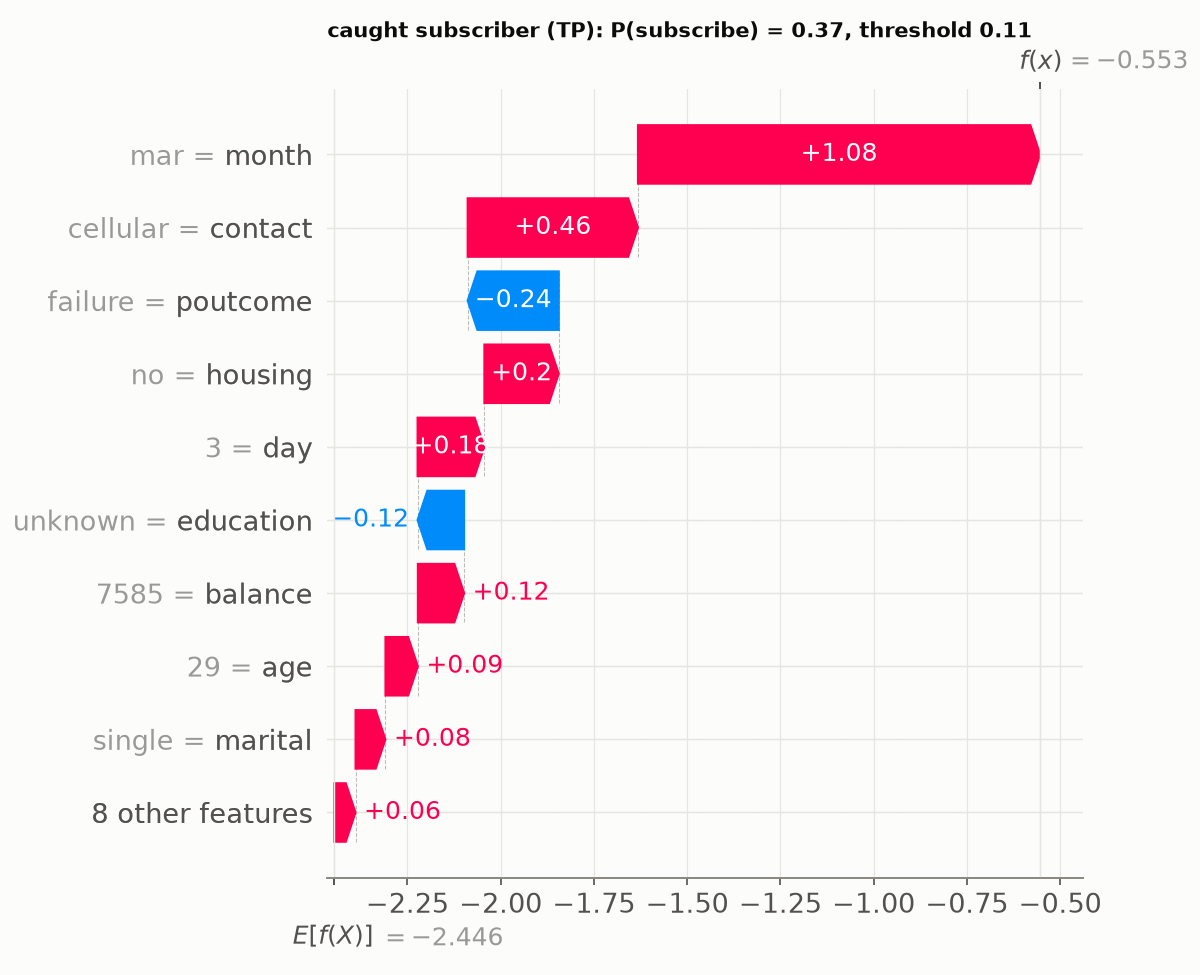
\includegraphics[width=\linewidth]{shap_local_TP}\end{subfigure}
\begin{subfigure}{0.49\textwidth}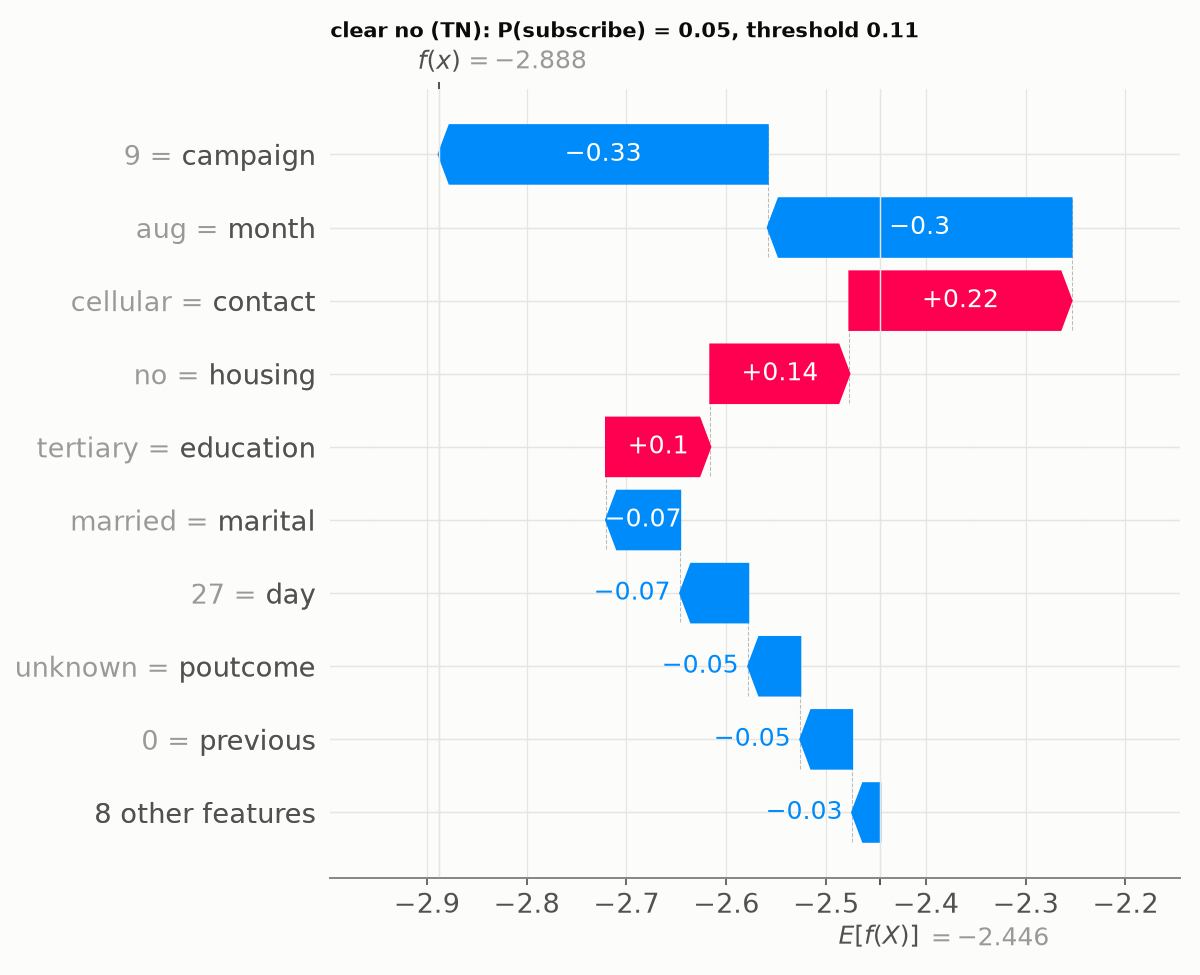
\includegraphics[width=\linewidth]{shap_local_TN}\end{subfigure}
\caption{Local SHAP. Left: caught subscriber (March, mobile). Right: clear ``no'' (9 calls, August).}
\end{figure}

\begin{figure}[H]
\centering
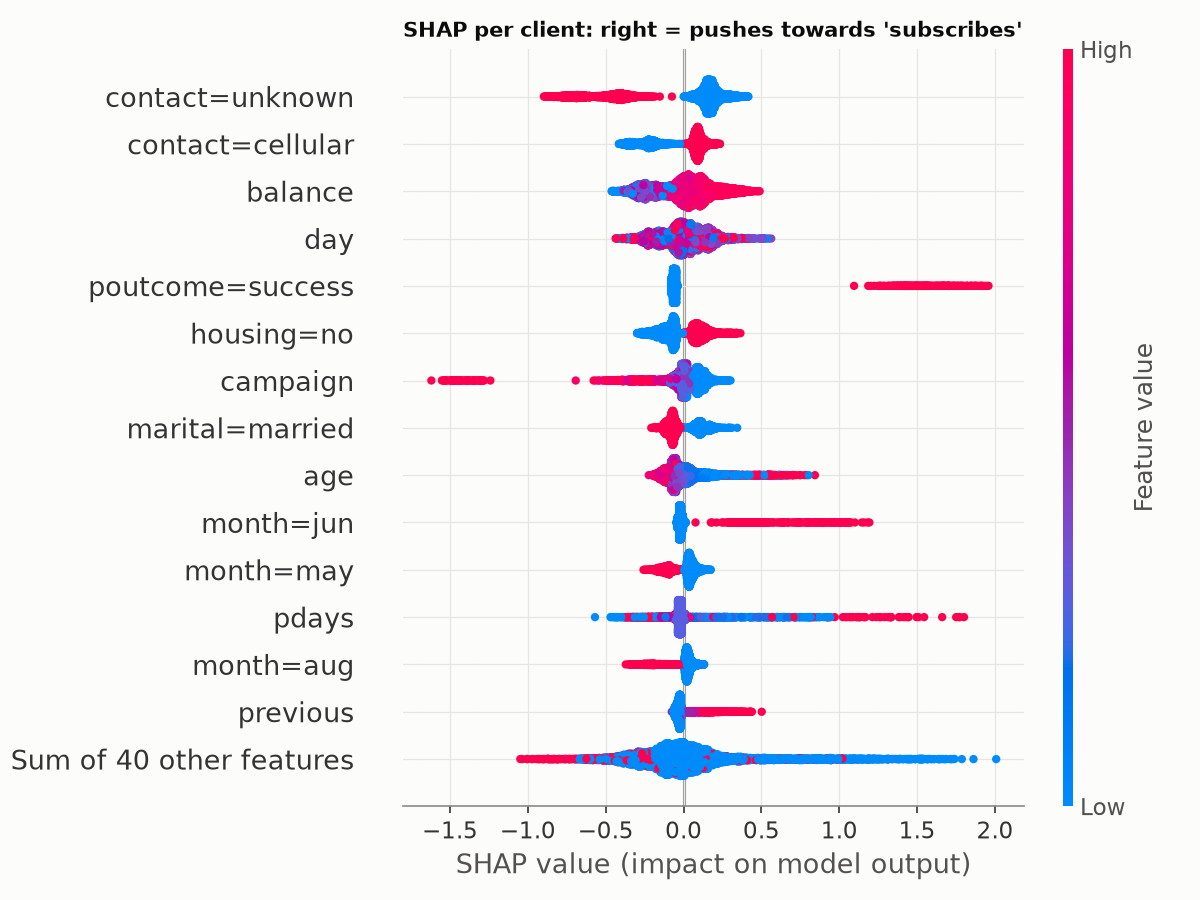
\includegraphics[width=0.6\textwidth]{shap_beeswarm}
\caption{SHAP beeswarm: one dot per client, colour = feature value.}
\end{figure}

\begin{figure}[H]
\centering
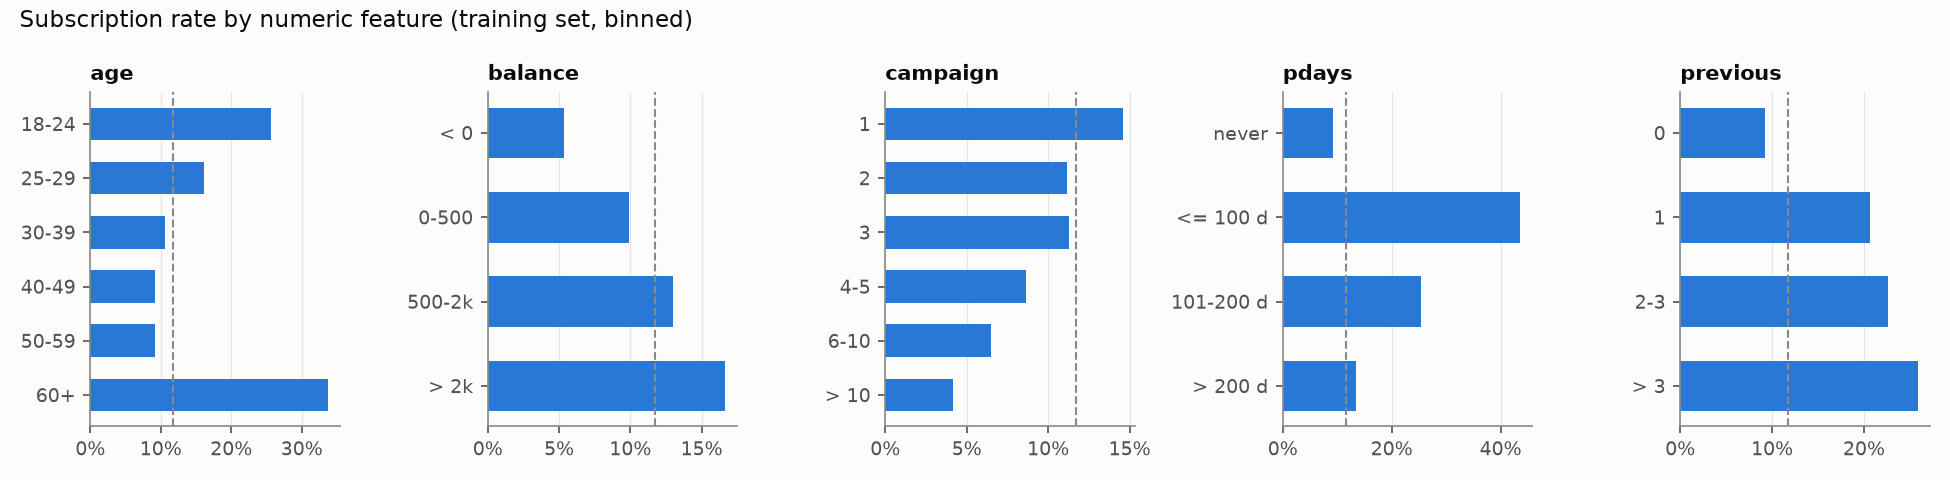
\includegraphics[width=0.95\textwidth]{eda_numeric_rates}
\caption{Subscription rate by binned numeric feature (training set).}
\end{figure}

\begin{figure}[H]
\centering
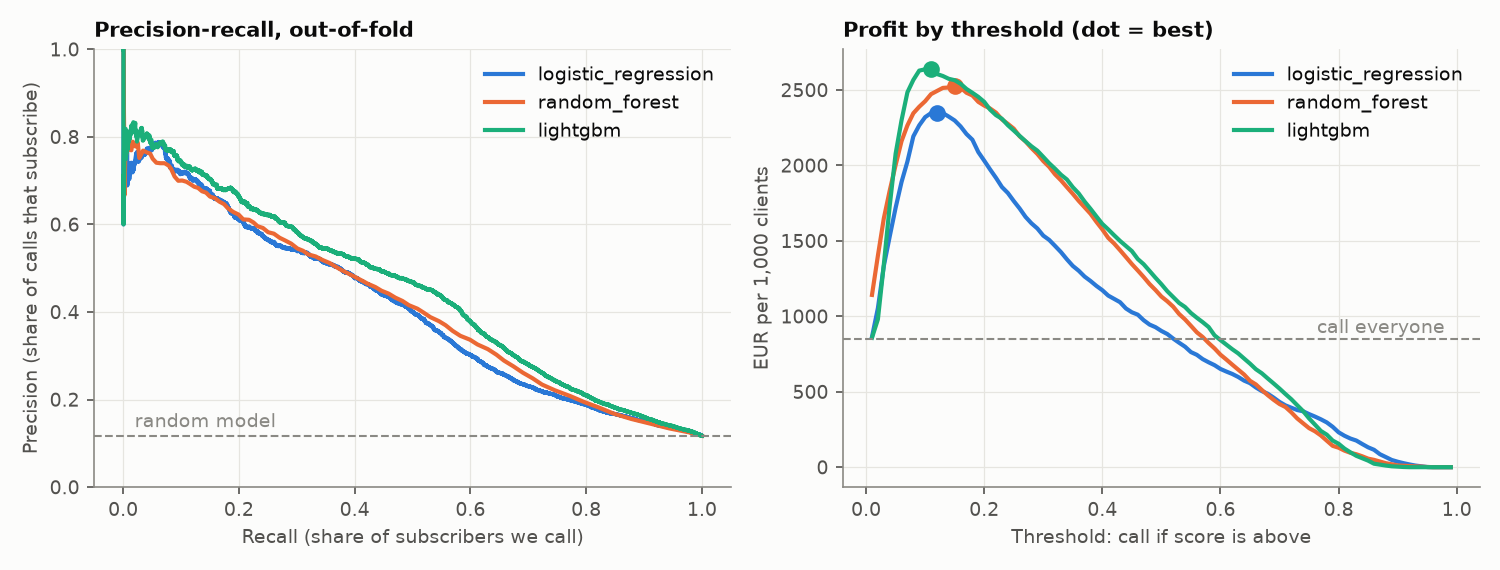
\includegraphics[width=0.9\textwidth]{models_pr_and_profit}
\caption{Precision--recall and profit curves of the three default models (CV).}
\end{figure}

\begin{figure}[H]
\centering
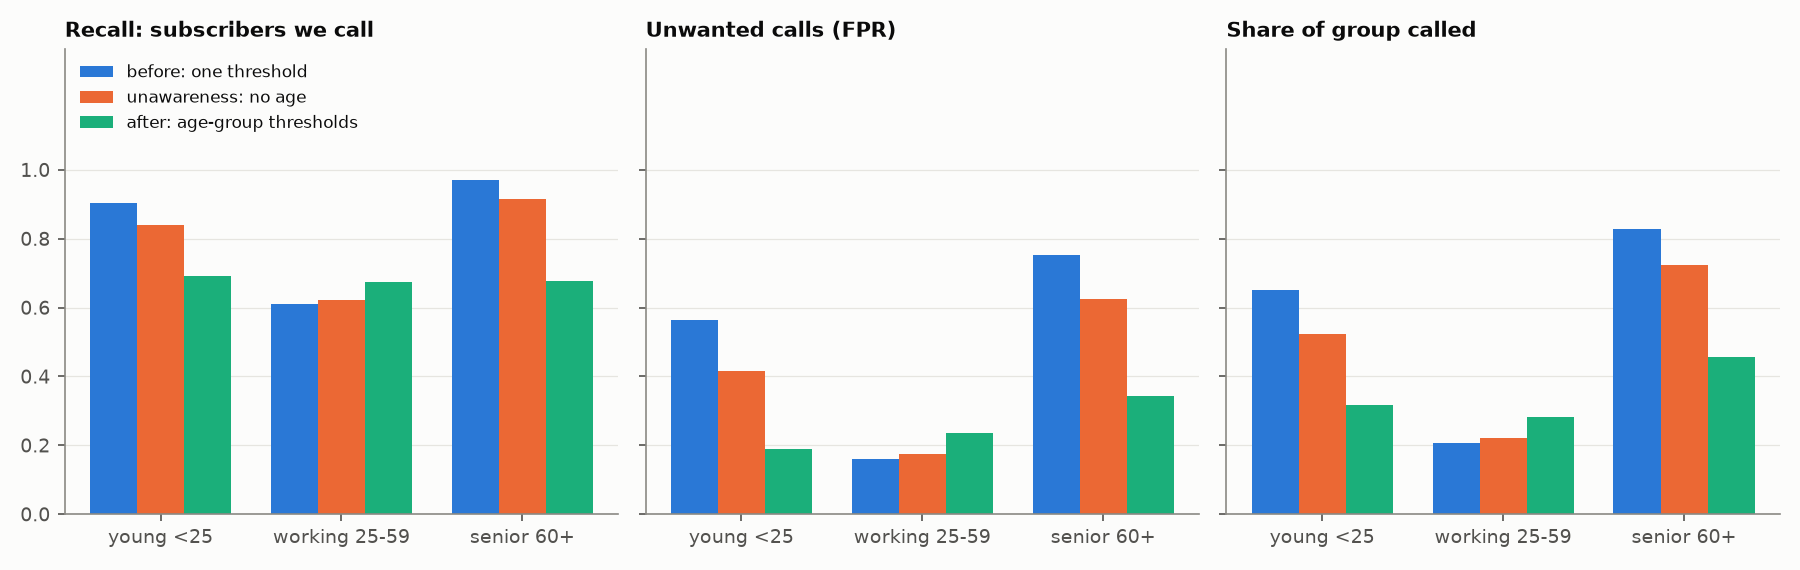
\includegraphics[width=0.92\textwidth]{fairness_cv}
\caption{Fairness on CV: one threshold, unawareness (no age), age-group thresholds.}
\end{figure}

\end{document}
